\documentclass[12pt, a4paper]{article}
\usepackage[margin=2.5cm]{geometry}
\usepackage[utf8]{inputenc}
\usepackage{color, amssymb}
\usepackage{listings, amsmath, float}
\renewcommand{\baselinestretch}{1.5}
\setlength\parindent{24pt}
\usepackage{graphicx}
\graphicspath{ {./images/} }

\title{Lab 1}
\author{Odysseas Stavrou}
\date{October 2020} 

\begin{document}
\noindent\rule{\textwidth}{1.5pt}

\begin{center}
{\bf Digital Signal Processing} \\ 
 1st Lab Exercise\\
 Odysseas Stavrou 2018030199\\
 Lab Group No: 90\\
 November 2020\\
 Technical University of Crete\\
\end{center}
\noindent\rule{\textwidth}{1.5pt}


\begin{enumerate}
    \item[1.]~
    \begin{enumerate}
        \item[A.]Convolution of 2 discrete signals with and without the conv() function.
        The 2 signals chosen were 2 discrete pulses \(x_1\) and \(x_2\):
        \[x_1 = u[n-1] - u[n-3]\]
        \[x_2 = u[n-3] - u[n-5] + u[n-7] - u[n-9]\]
        \[n \in [\,0,9.8]\,\ with\ a\ step\ of\ 0.2\]

        \begin{figure}[H]
            \centering
            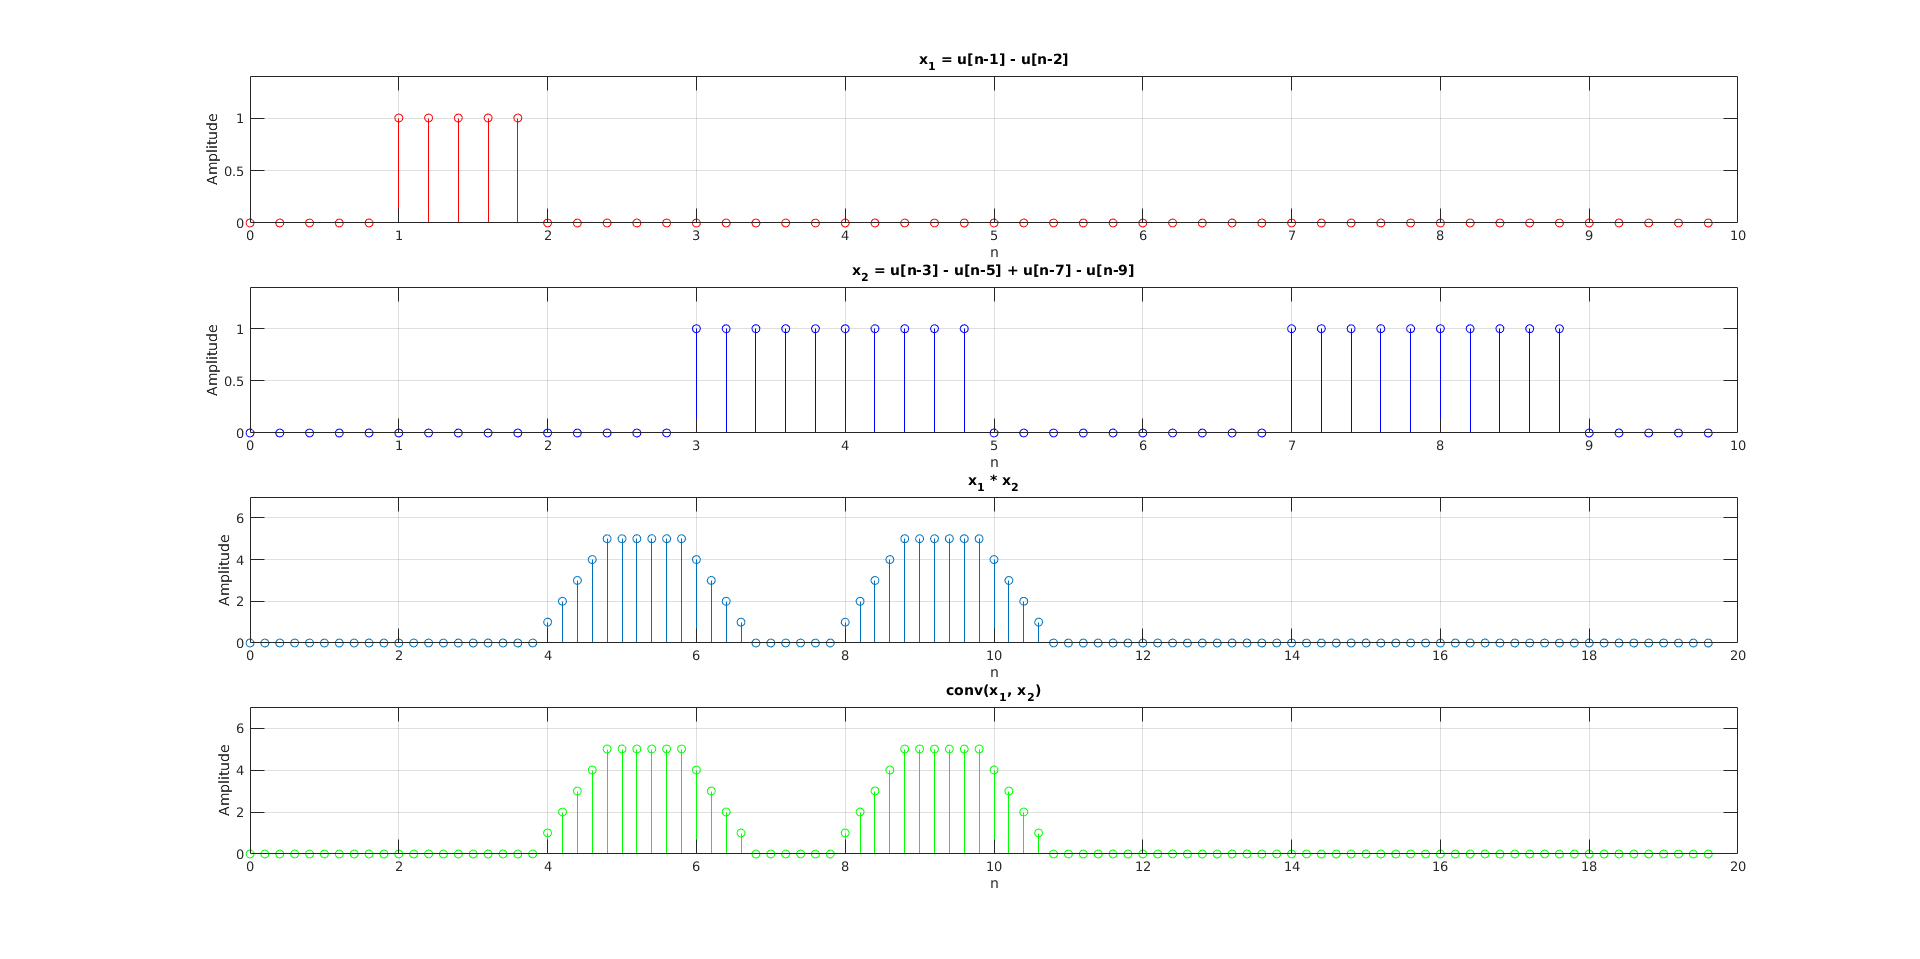
\includegraphics[width=\textwidth, height=9cm]{A_1.png}
            \caption{The 2 signals \(x_1\) and \(x_2\) and their convolution, from scratch and by using MATLAB's built in function, respectively}
        \end{figure}

        \item[B.]Proof of properties of Convolution and the Fourier Transform
        \[x_1[n] \circledast x_2[n] = X_1[N] \cdot X_2[N]\]
        In order to prove the above property we need to calculate the FT of both signals and then multiply them together.
        We already have the convolution from the above question, but in the wrong field. We need to calculate the FT of the 
        Convolution as well to bring them both in the same field. (Note: We can also calculate the inverse FT of the product
        insted of transforming the convolution)
        \begin{figure}[H]
            \centering
            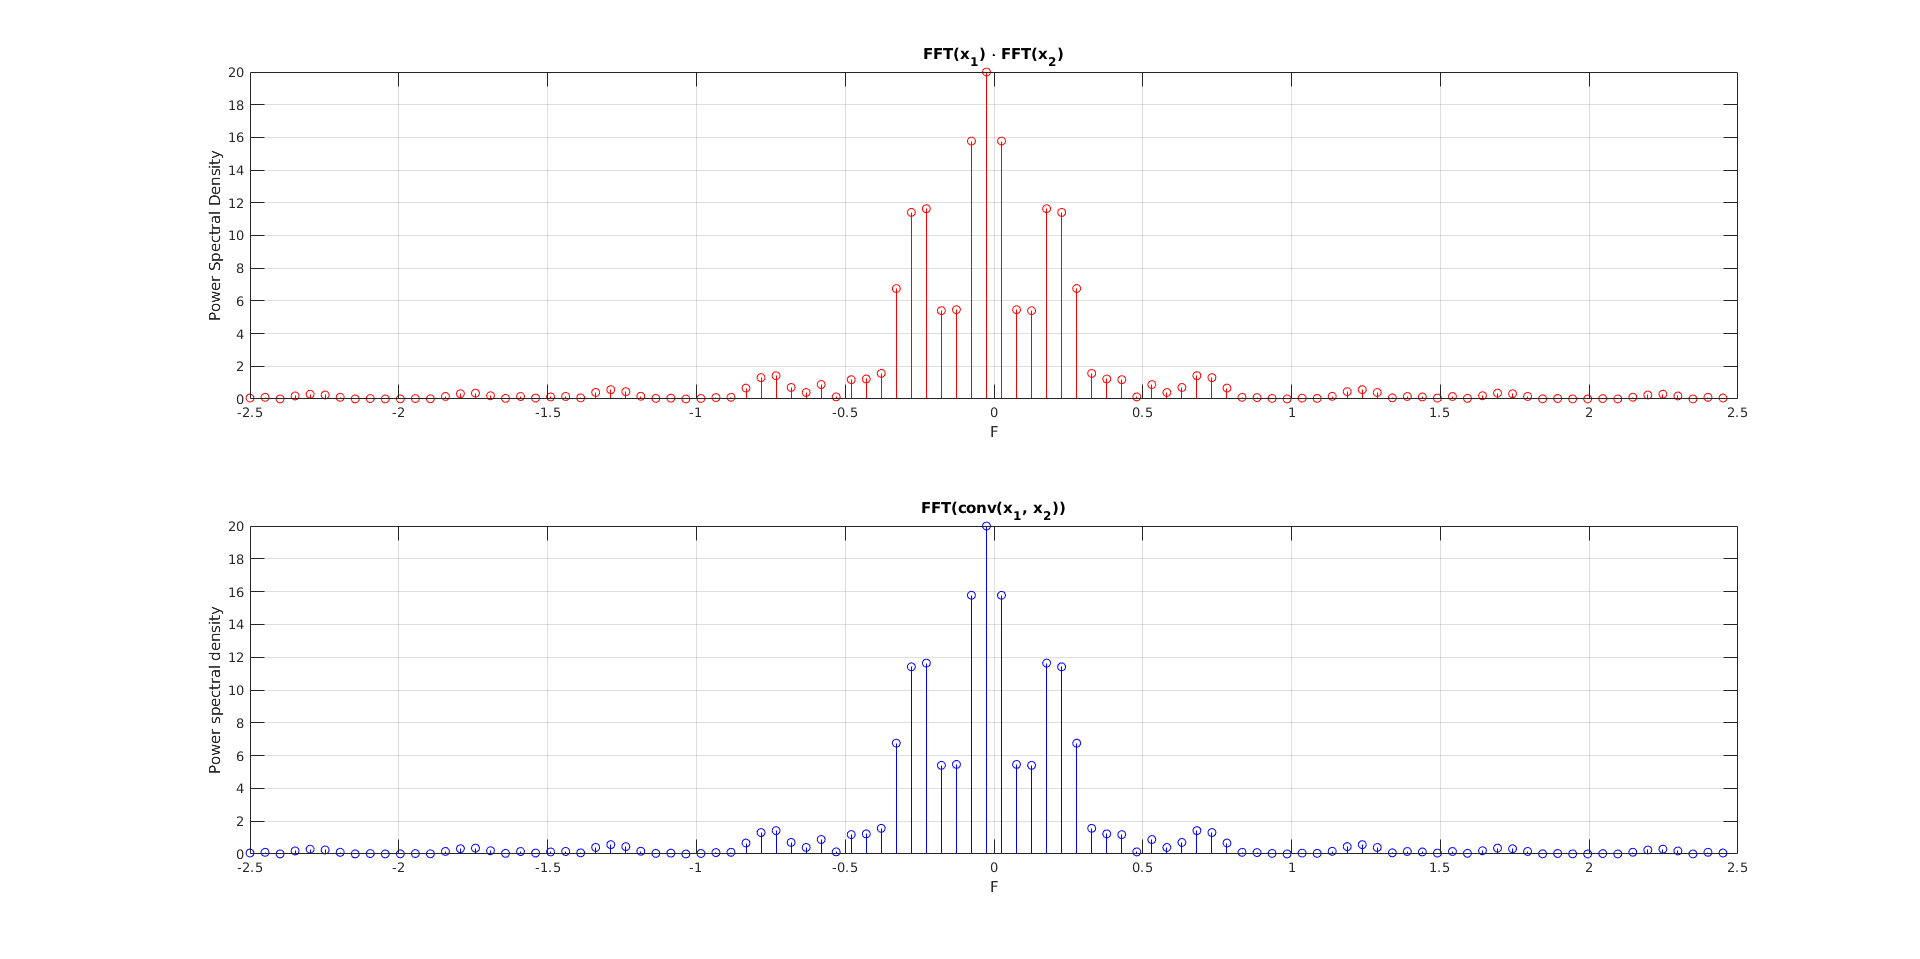
\includegraphics[width=\textwidth, height=10cm]{B_1.png}
            \caption{Multiplying the FFTs of both signals vs.\ taking the FFT of their convolution from earlier}
        \end{figure}
        
    \end{enumerate}
    \item[2.] 
    Fourier Transform (on paper) the following signal and sample it using the following frequencies:
    \[x(t) = 5\cos(2\pi12t) - 2\sin(2\pi\frac{3}{4}t)\]
    \begin{enumerate}
        \item[a.] \(f_s = 48Hz\)
        \item[b.] \(f_s = 24Hz\)
        \item[c.] \(f_s = 12Hz\)
        \item[d.] \(f_s = 90Hz\)
    \end{enumerate}

    \begin{enumerate}
        \item[i.] To calculate the Nyquist frequency we need to take the largest frequency (\(f_{\max}\)) of our two signals in this case \(12Hz\).
        Nyquist's frequency is the lowest sampling frequency of a signal that can reconstruct the original. Sampling with any 
        frequency lower than this, will render the reconstruction worthless.
        \[f_{nyq} = 2 * f_{\max} = 2 * 12 Hz = 24Hz\]

        \item[ii.] Using the complex identities of the sine and cosine functions we can easily derive a sequence of terms for the above mentioned signal:
        \[\cos(t) = \frac{e^{jt} + e^{-jt}}{2}\]
        \[\sin(t) = \frac{e^{jt} - e^{-jt}}{2j}\]
        \[x(t) = \frac{5}{2}e^{2\pi j12t} + \frac{5}{2}e^{-2\pi j12t} + je^{-2\pi j\frac{3}{4}t}
        -je^{2\pi j\frac{3}{4}t}\]

        
        \item[iii.] Transforming each term from above and using the time/frequency shift properties of the FT:
        \[F\{ \delta \}=1\]
        \[x_{a}e^{2\pi jft} = X(F-f)\]
        we end up with:
        \[X(F) = \frac{5}{2}\delta(F-12) + \frac{5}{2}\delta(F+12) + 
        j\delta(F+\frac{3}{4}) - j\delta(F-\frac{3}{4})\]

        \item[iv.] As seen below, sampling with \(f_{\max}\) does not produce enough information for us to 
        be able to reconstruct the signal, where as in sampling with twice the \(f_{\max}\) yields just bearly enough information
        about the signal. Taking samples with any frequency \(>f_{\max}\), will result in a better resolution and of course 
        more samples. In my case the last sampling frequency is \(90Hz\) which is more that enough.

        \begin{figure}[H]
            \centering
            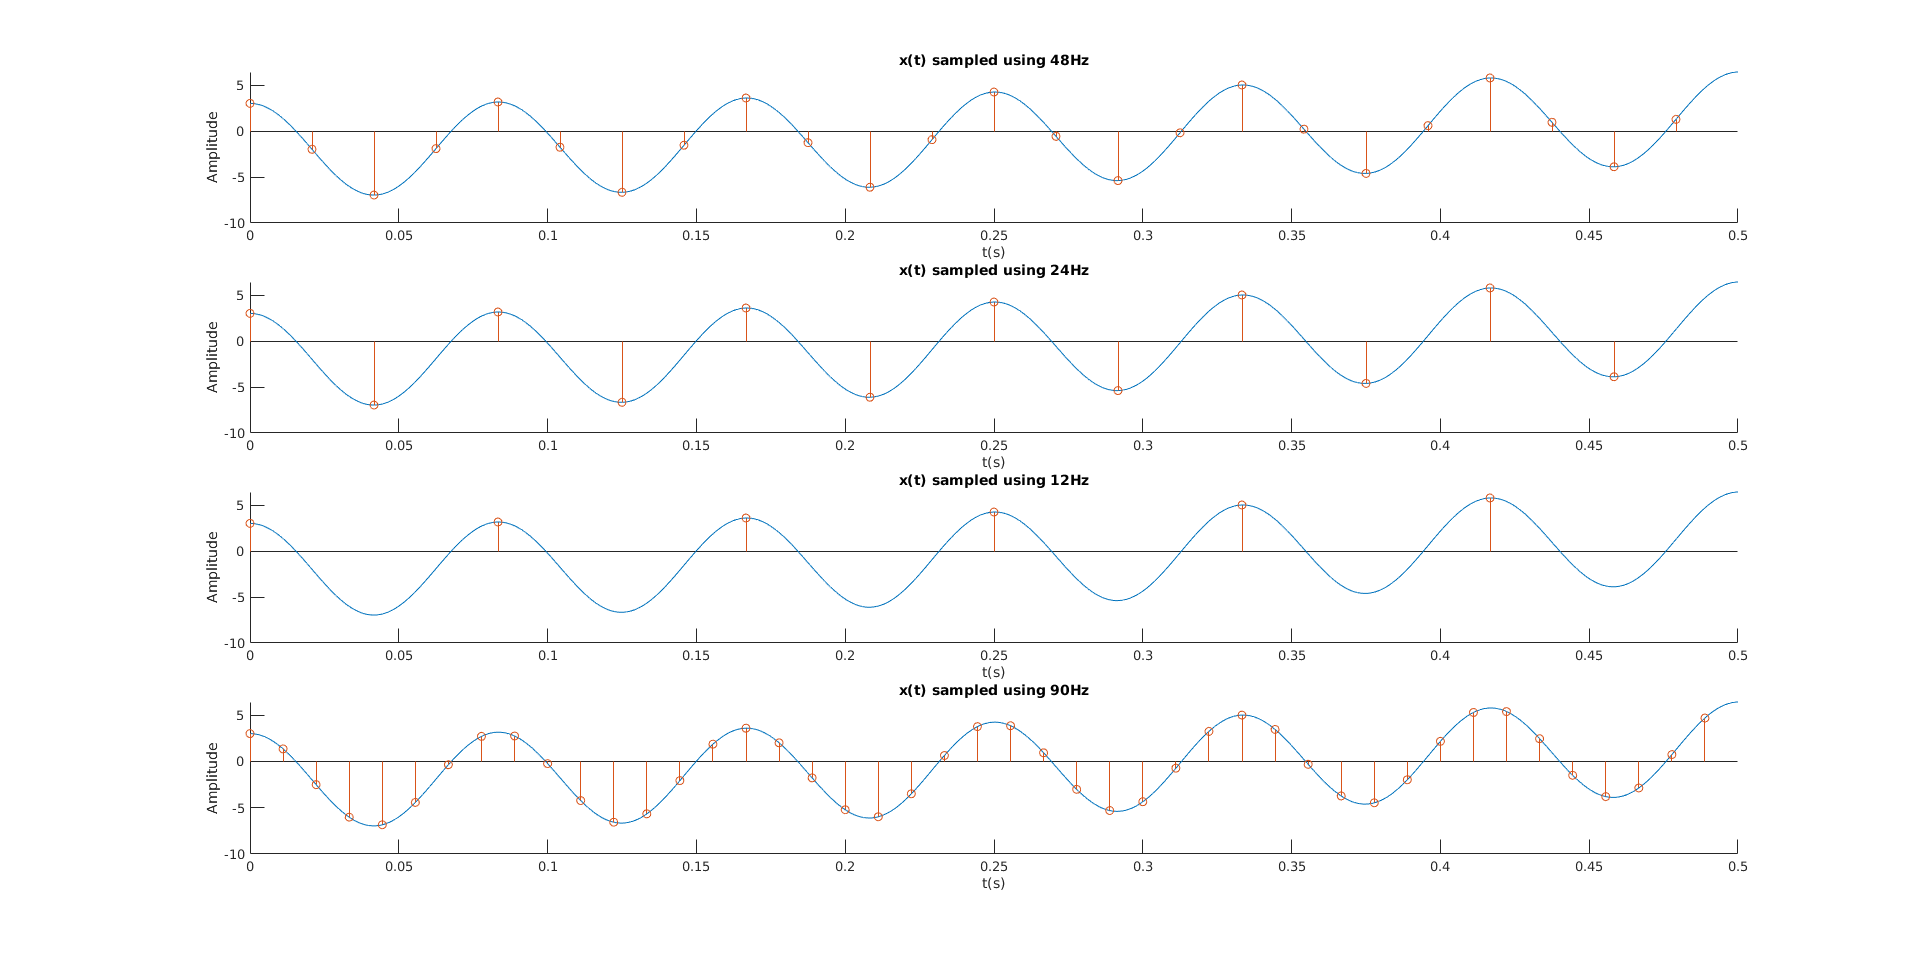
\includegraphics[width=\textwidth, height=10cm]{2.png}
            \caption{Sampling of \(x(t)\) using different frequencies}
        \end{figure}
    \end{enumerate}
    \pagebreak
    \item[3.]~
    \begin{enumerate}
        \item[A.] Capture 128 samples of the following signal and display the signal into the frequency spectrum
        \[x(t) = 10\cos(2\pi20t) - 4\sin(2\pi40t)\] with a frequency such that, the aliasing effect is not visible.

        Using: 
        \[f_{sampl} \geqslant f_{nyq} = 2 * f_{\max} \Rightarrow f_{sampl} \geqslant 80 Hz\]
        Chosen:
        \[f_{sampl} = 500 Hz\]

        We can observe peaks in the frequency spectrum at the positive and negative frequencies of the two signals 
        used to create \(x(t)\).\\
        Peaks at: 
        \begin{enumerate}
            \item[i.] \(-f_1 = -20Hz\), \(f_1 = 20Hz\)
            \item[ii.] \(-f_2 = -40Hz\), \(f_2 = 40Hz\)
        \end{enumerate}
        \begin{figure}[H]
            \centering
            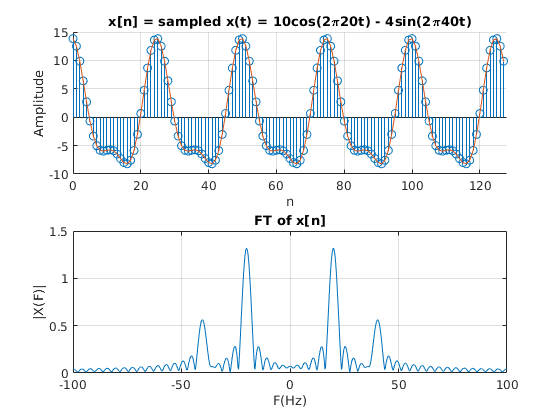
\includegraphics[width=\textwidth, height=10cm]{3_A.png}
            \caption{Sampling of \(x(t)\) and its frequency spectrum}
        \end{figure}
        \item[B.] Define the following signal:
        \[x(t) = \sin(2\pi f_0t + \phi)\]
        Sampling the above signal with a SF (\(f_{s}\)) of 8KHz and by using this property:
        \[x[n] = x_a(nT_s) = x_a(n\frac{1}{f_s})\]
        the resulting discrete signal is:
        \[x[n] = \sin(2\pi \frac{f_0}{f_{s}} n + \phi)\]
        \item[i.] Plotting for all 4 (low) (\(100Hz - 475Hz, step=125Hz\)) different sinusodial frequencies we get the following spectrum for each:   
        \begin{figure}[H]
            \centering
            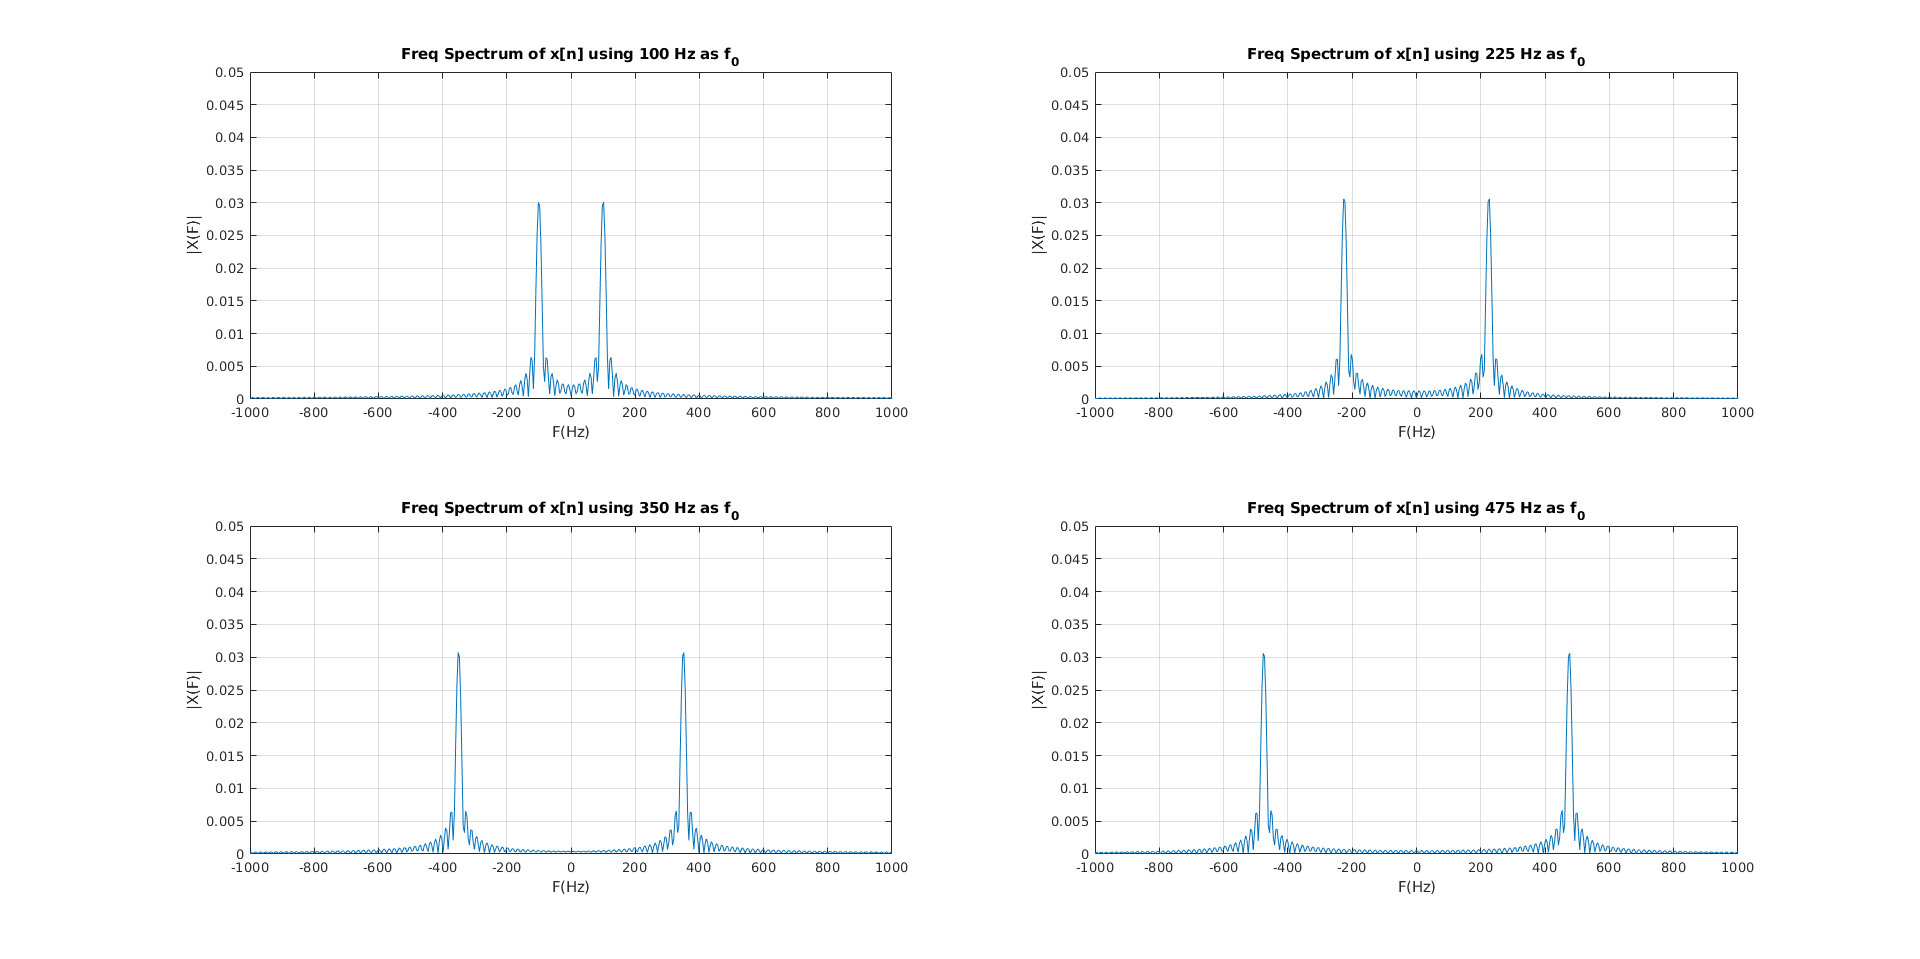
\includegraphics[width=\textwidth, height=10cm]{3_B_1.png}
            \caption{Frequency Spectrum of \(x(t)\)}
        \end{figure}
    \end{enumerate}
    We can observe that, because the SF, \(f_s\), is so high in respect to \(f_0\) the peaks are shown at every \(f_0\)
    point on the Frequency Spectrum which is expected, since that is the Frequency of our sinusodial wave.
    \pagebreak
    \begin{enumerate}
        \item[ii.]Plotting for all 4 (high) (\(7525Hz - 7900Hz, step=125Hz\)) different sinusodial frequencies we get the following spectrum for each:   
        \begin{figure}[H]
            \centering
            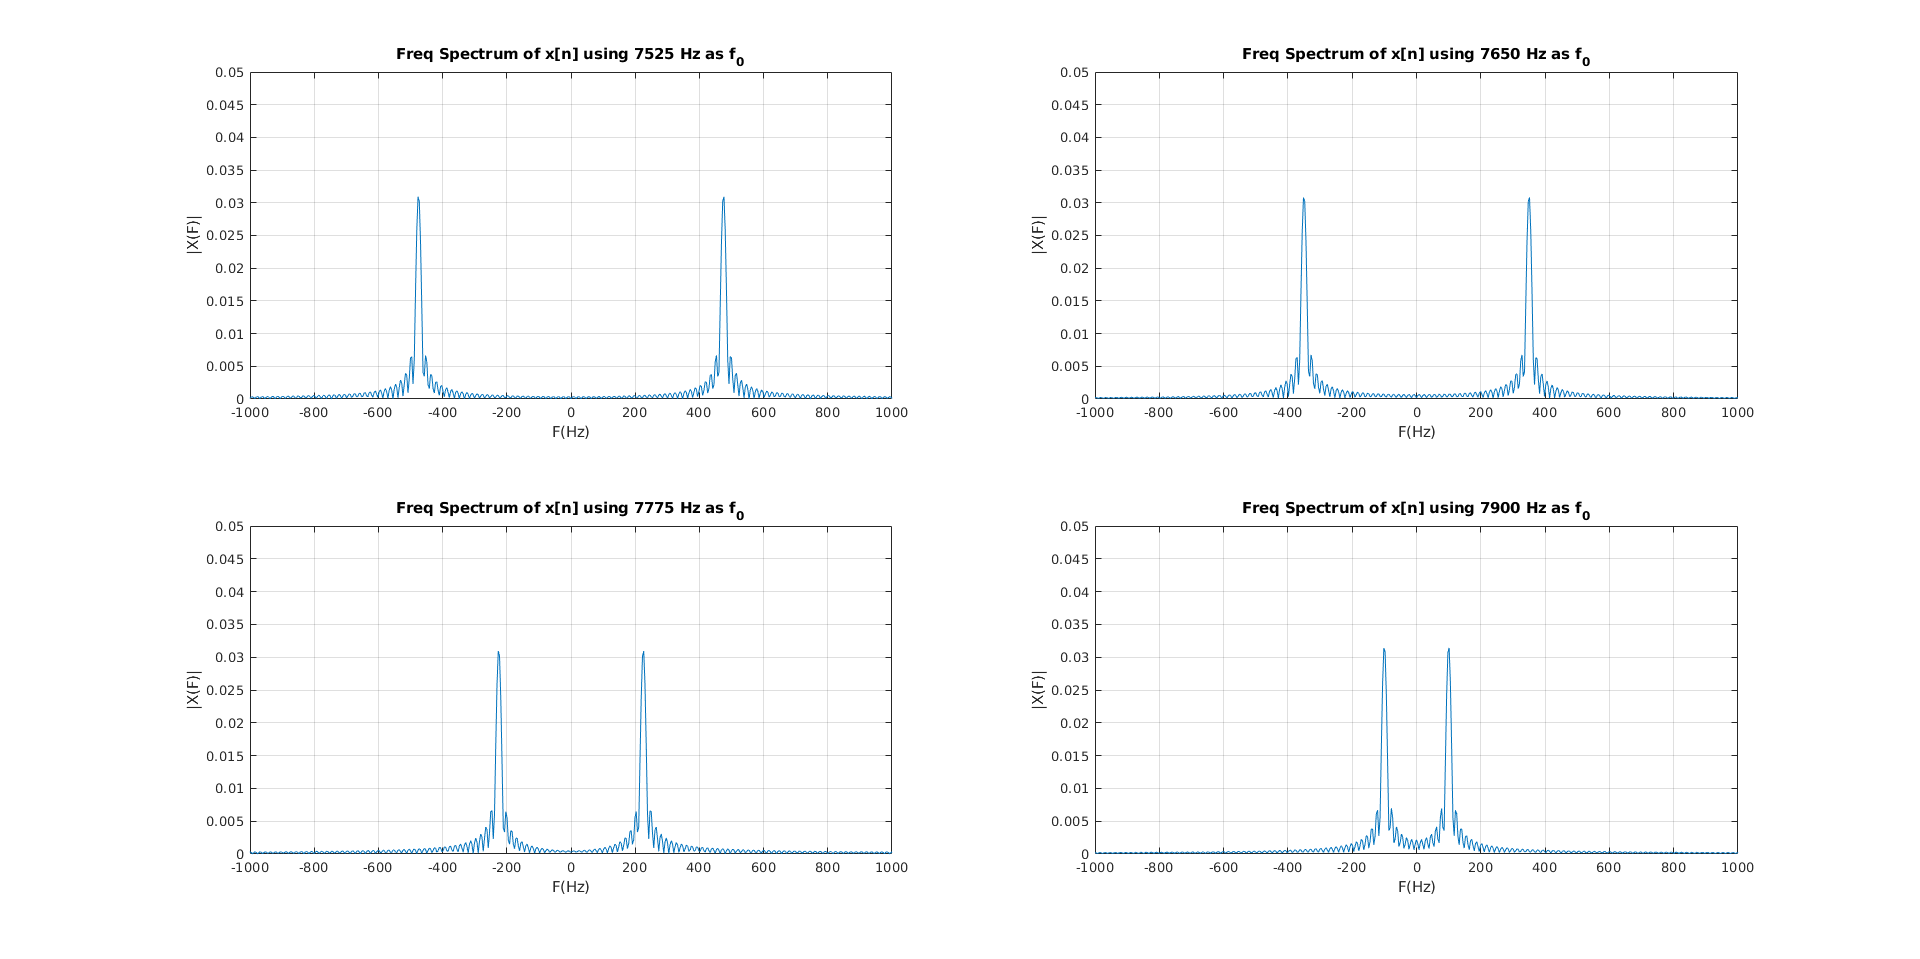
\includegraphics[width=\textwidth, height=10cm]{3_B_2.png}
            \caption{Frequency Spectrum of \(x(t)\)}
        \end{figure}
    \end{enumerate}
    However in this case the peaks exist at points \(f_0 - f_s\). This is happening because the SF \(f_s\) is bellow the Nyquist
    limit. This is called the aliasing effect, because the sinusodial wave, clearly, has a way larger Frequency than before but, despite 
    that, the signal that ``seems'' to be sampled is a signal with a Frequency of \(f_0 - f_s\) and not \(f_0\).
    Changing the starting phase \(\phi \) will have no effect what so ever, because \(\phi \) is just a starting offset, and does not mess with 
    the Frequency.
\end{enumerate}
\end{document}